\begin{surferPage}[Sextica de 30 Picos]{La Séxtica de Barth de 30 picos}
    Wolf Barth ya había construido la séxtica con la mayor cantidad de
    singularidades posibles, $65$ (ver la otra superficie de Barth
    en esta galería), y además dos de sus estudiantes de doctorado habían
    construido otro mundo de superficies récord, para grados más altos.
    Pero para él, esto fue sólo una motivación para llegar a otra pregunta:
    ¿Cuál es el máximo de picos que puede tener una superficie, sabiendo su grado?

   La construcción de la séxtica de Barth de $65$ singularidades del tipo doble cono,
   puede ser adaptada a picos. Esta modificación nos deja $30$ de ellos: 
    \[P_6 - \alpha \cdot K^3=0,\]
  donde $P_6$ es el mismo plano simétrico del icosaedro que la otra séxtica de Barth,
  y donde $K$ es, otra vez, la ecuación de la esfera unitaria:
    \vspace*{-0.4em}
    \begin{center}
      \begin{tabular}{c@{\ }c@{\ }c@{\ }c}
        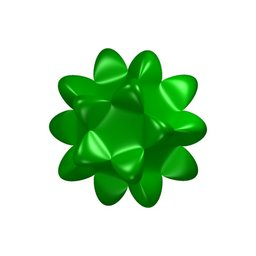
\includegraphics[height=1.2cm]{barthsextic_30A2}
        &
        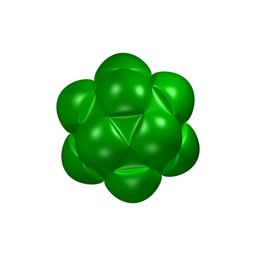
\includegraphics[height=1.2cm]{barthsextic_30A2_3}
        &
        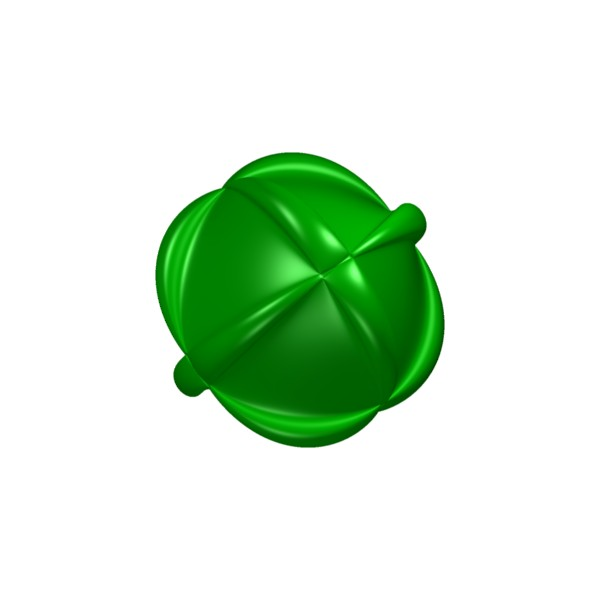
\includegraphics[height=1.2cm]{barthsextic_30A2_5}
        &
        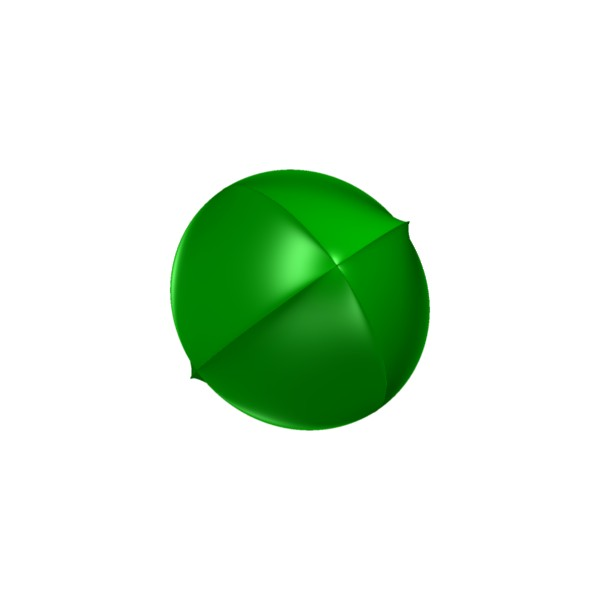
\includegraphics[height=1.2cm]{barthsextic_30A2_6}
      \end{tabular}
    \end{center}    
    \vspace*{-0.3em}
     Este es el actual récord mundial en cantidad de picos reales en séxticas.
     Para picos complejos es $36$.
\end{surferPage}
